\graphicspath{ {Figures/Pileup/Multiplier/} {Figures/Pileup/Phase/} {Figures/RandomSeeds/FitStartScans/} {Figures/RandomSeeds/FitIterations/} }

\chapter{Systematic Uncertainty Evaluations}

\section{Sensitivity of \texorpdfstring{$\omega_{a}$}{} to gain corrections}

\section{Sensitivity of \texorpdfstring{$\omega_{a}$}{} to pileup}

The systematic error on R due to the pileup construction consists primarily of two parts, the error due to misconstruction of the amplitude and the phase of the pileup. The error due to the amplitude misconstruction was calculated by scanning over a pileup multiplier parameter, from 90\% of the calculated pileup amplitude to 110\%, as shown in Figure \ref{fig:PileupMultiplier}. The sensitivity of R to the amplitude was determined to be 509.1 ppb per unit amplitude. The uncertainty of the pileup amplitude construction was determined by fitting a parabola to the \chisq as a function of the pileup amplitude, and taking the width of that parabola as the uncertainty. This width is determined as the distance in X for the \chisq to rise by 1 from the minimum, also calculated as $\sqrt{2/(\chi^{2})''}$.

\begin{figure}[H]
\centering
    \begin{subfigure}[t]{0.45\textwidth}
	    \centering
		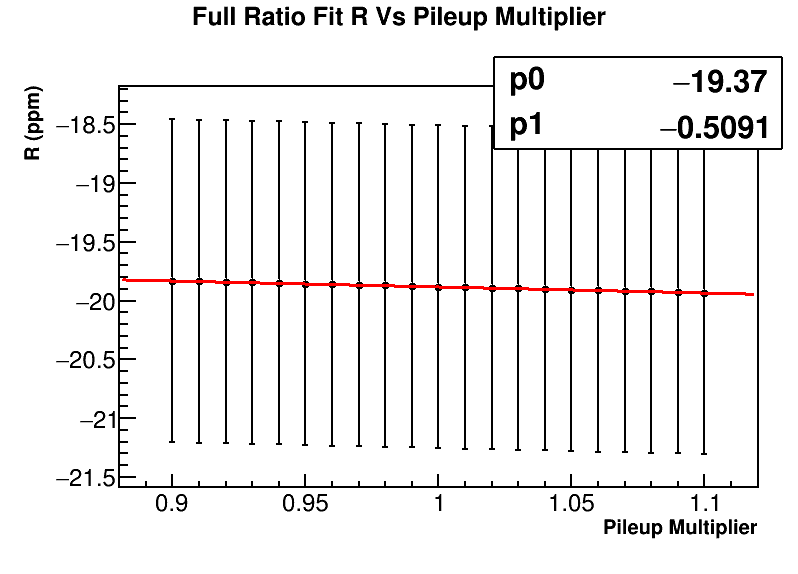
\includegraphics[width=\textwidth]{RatioCBO_R_Vs_PileupMultiplier_Canv}
	    \caption{Sensitivity of R vs the pileup amplitude. The slope is -509.1 ppb per unit amplitude.}
    \end{subfigure}
    \hspace{4mm}
    \begin{subfigure}[t]{0.45\textwidth}
	    \centering
		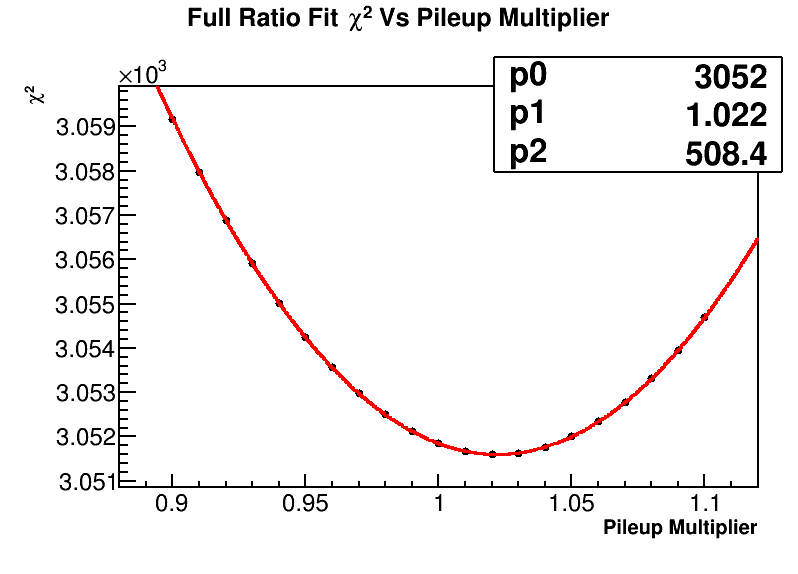
\includegraphics[width=\textwidth]{RatioCBO_Chi2_Vs_PileupMultiplier_Canv}
	    \caption{Plotted is the fitted \chisq vs the pileup amplitude. The fit equation used was $p2 \times (x - p1)^{2} + p0.$ The minimum therefore lies at 1.022.}
    \end{subfigure}
\caption[PileupMultiplier]{The significant plots to determine the pileup amplitude systematic error.}
\label{fig:PileupMultiplier}
\end{figure}

This corresponds to an uncertainty of $\sqrt{1/508.4} = 0.0444$ or 4.44\%. The minimum of the \chisq plot of 1.022 lies at approximately .5$\sigma$ away from 1, which is consistent and nice to see. Then, calculating the systematic error on R due to the pileup amplitude construction as 
	\begin{align}
		\delta R_{pm} = \delta\alpha_{pm} \times \frac{dR}{d\alpha_{pm}}
	\end{align}
where $\delta\alpha_{pm}$ is the uncertainty on the pileup amplitude, the systematic error on R is calculated as 509.1 pbb $\times 0.0444 = 22.6$ ppb.

Another technique to estimate the uncertainty of the pileup amplitude construction is to look at the offset of the high energy tail of the pileup subtracted energy spectrum from zero. Because however I've applied only the doublet correction, I know that the shape of the pileup spectrum is wrong by some amount, as evidenced in \ref{fig:AddedEnergies}. While the pileup itself can multiplied by some scaling factor other than 1 in order to align the energy spectra slightly better, because the shape of the pileup correction is imperfect the offset calculation I believe is the wrong way to go about calculating this uncertainty in my case. The shape can be fixed by including the triplets and the doublet contamination in the shadow method, but that work is incomplete. Since the triplets are a 1\% effect relative to the doublets, and the contamination is of the same order, I believe the uncertainty of 4.44\% conservatively includes for this mismatch in shape and the omission of the triplets. Regardless, since the statistics of the 60H dataset is much larger than the order of the systematic effect for the pileup construction ($\mathcal{O}$(1 ppm) vs $\mathcal{O}$(10 ppb)), this is a fine assumption.

\begin{figure}[h]
	\centering
	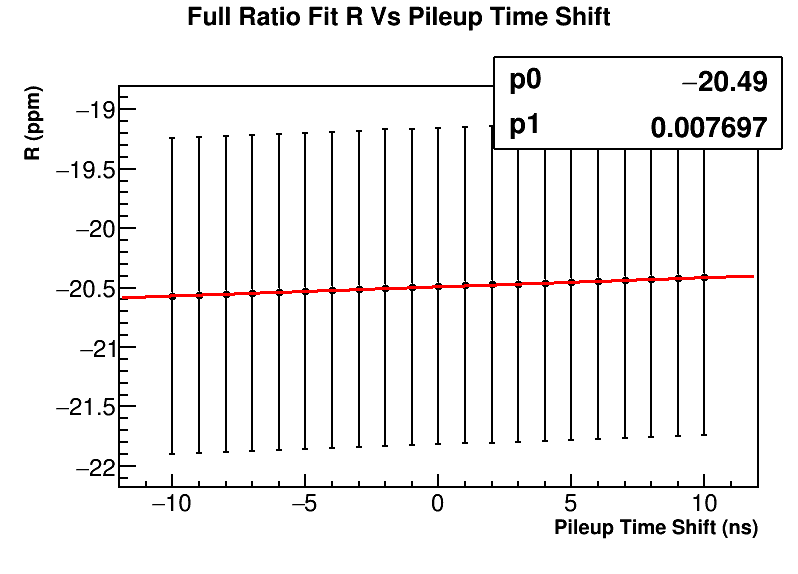
\includegraphics[width=.5\textwidth]{RatioCBO_R_Vs_PileupTimeShift_Canv}
    \caption[PileupPhase]{Sensitivity of R vs the pileup phase. The slope is 8.571 ppb per ns.}
    \label{fig:PileupPhase}
\end{figure}

The error on R due to the pileup phase construction was calculated by scanning over a pileup time shift parameter, where the pileup spectrum was shifted in time by some amount before subtraction. The sensitivity of R to this parameter is shown in Figure \ref{fig:PileupPhase}. It is extremely unlikely that the entire pileup spectrum could be shifted by the offsets shown here, so this is a conservative estimate of the effect of the pileup phase on R. Another factor that the phase depends on is the energy dependence of the constructed pileup pulses, calculated as just the sum of the singlets. If the energy is miscalculated then the phase of the included pulses will be off. However, because the spatial separation is turned off in the reconstruction clustering, this is a small effect for my pileup construction method. Similarly, in the near future the Short Term Double Pulse (STDP) improvement to the laser calibration will be included also reducing this effect. For these reasons and due to the conservative nature of my phase error estimation, I leave such effects out. I then calculate the phase error as 
	\begin{align}
		\delta R_{pp} = \delta\alpha_{pp} \times \frac{dR}{d\alpha_{pp}}
	\end{align}
where $\delta\alpha_{pp}$ is the uncertainty on the pileup phase. I once again very conservatively estimate the uncertainty on the pileup phase as half the artificial deadtime at 3ns. The systematic error on R is then calculated as 8.571 pbb $\times 3 = 25.7$ ppb. This is a very conservative estimate which is fine once again because of the comparison of order of statistics vs the systematic effect.

\begin{figure}[]
	\centering
	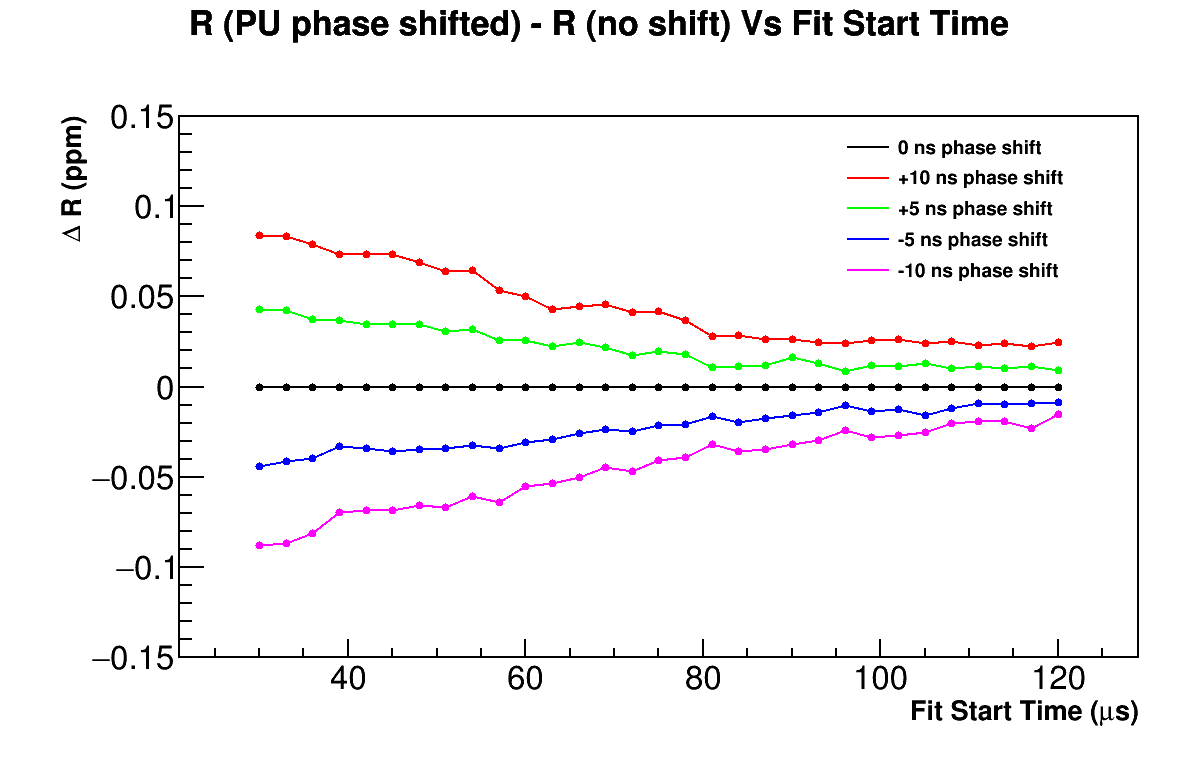
\includegraphics[width=.8\textwidth]{pileupTimeShiftComparison}
    \caption[PileupTimeShiftFS]{Plotted is $\Delta R$ between pileup time shifted and unshifted results vs fit start time. The black line and points are by definition 0. As the fit start time increases and the pileup reduces, the $\Delta R$ points converge to zero as they should.}
    \label{fig:PileupTimeShiftFS}
\end{figure}

Adding these two errors in quadrature results in a systematic error on R due to the pileup as 34.2 ppb.



\section{Sensitivity of \texorpdfstring{$\omega_{a}$}{} to lost muon function shape}

\section{Sensitivity of \texorpdfstring{$\omega_{a}$}{} to CBO function}

\section{Sensitivity of \texorpdfstring{$\omega_{a}$}{} to VW function}

\section{Sensitivity of \texorpdfstring{$\omega_{a}$}{} to various effects}

\subsection{Randomization}

I'm not sure what the systematic error due to the randomization should be. I'm also not sure what I should take as my final answer for R. Would it just be the average of all the random seeds?

\begin{figure}[]
\centering
    \begin{subfigure}[t]{0.45\textwidth}
	    \centering
		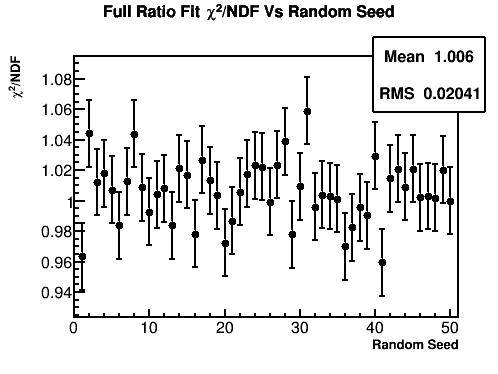
\includegraphics[width=\textwidth]{RatioCBO_Chi2NDF_Vs_Iter_Canv}
	    \caption{\chisq/NDF vs random seed number.}
    \end{subfigure}
    \begin{subfigure}[t]{0.45\textwidth}
	    \centering
		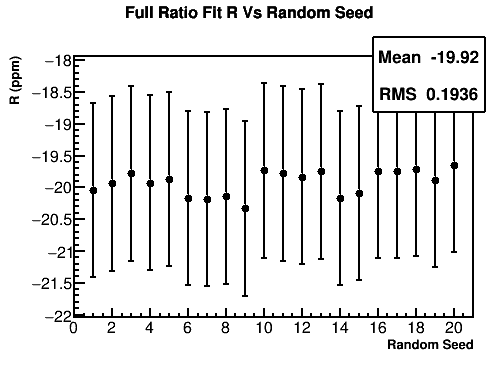
\includegraphics[width=\textwidth]{RatioCBO_R_Vs_Iter_Canv}
	    \caption{R vs random seed number.}
    \end{subfigure}% %you need this % here to add spacing between subfigures
\caption[RandomSeeds]{Plotted is the \chisq/NDF and fitted R value for 20 random seeds.}
\label{fig:RandomSeeds}
\end{figure}

\begin{figure}[]
\centering
    \begin{subfigure}[t]{0.45\textwidth}
	    \centering
		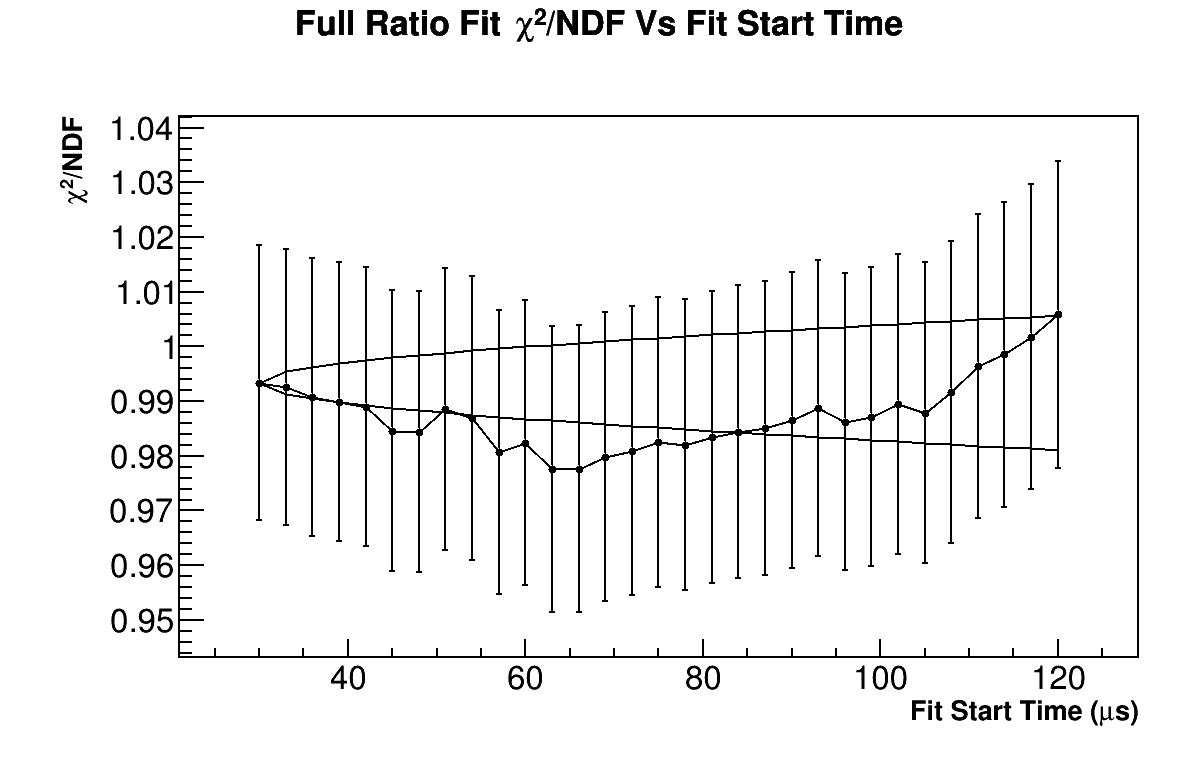
\includegraphics[width=\textwidth]{RatioCBO_Chi2NDF_Vs_FS_canv-Seed0}
	    \caption{Seed 1}
    \end{subfigure}
    \begin{subfigure}[t]{0.45\textwidth}
	    \centering
		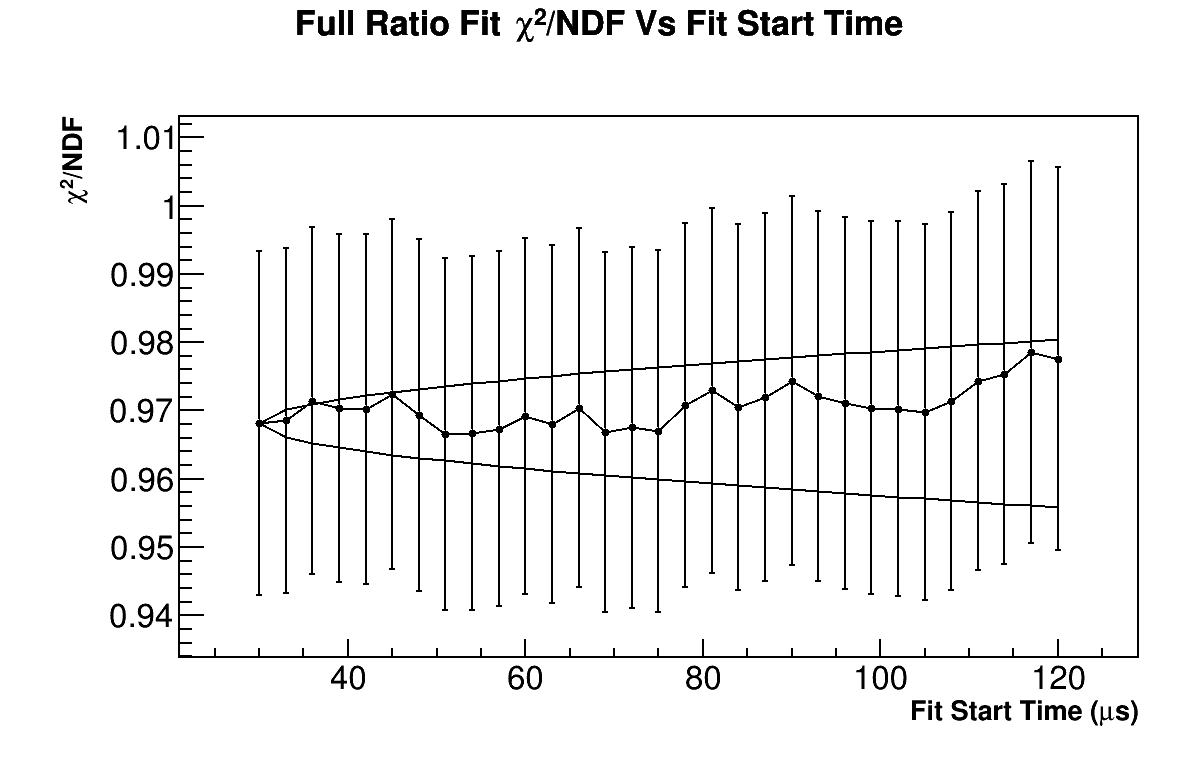
\includegraphics[width=\textwidth]{RatioCBO_Chi2NDF_Vs_FS_canv-Seed5}
	    \caption{Seed 2}
    \end{subfigure}% %you need this % here to add spacing between subfigures
    \vspace{4mm}
    \begin{subfigure}[t]{0.45\textwidth}
	    \centering
		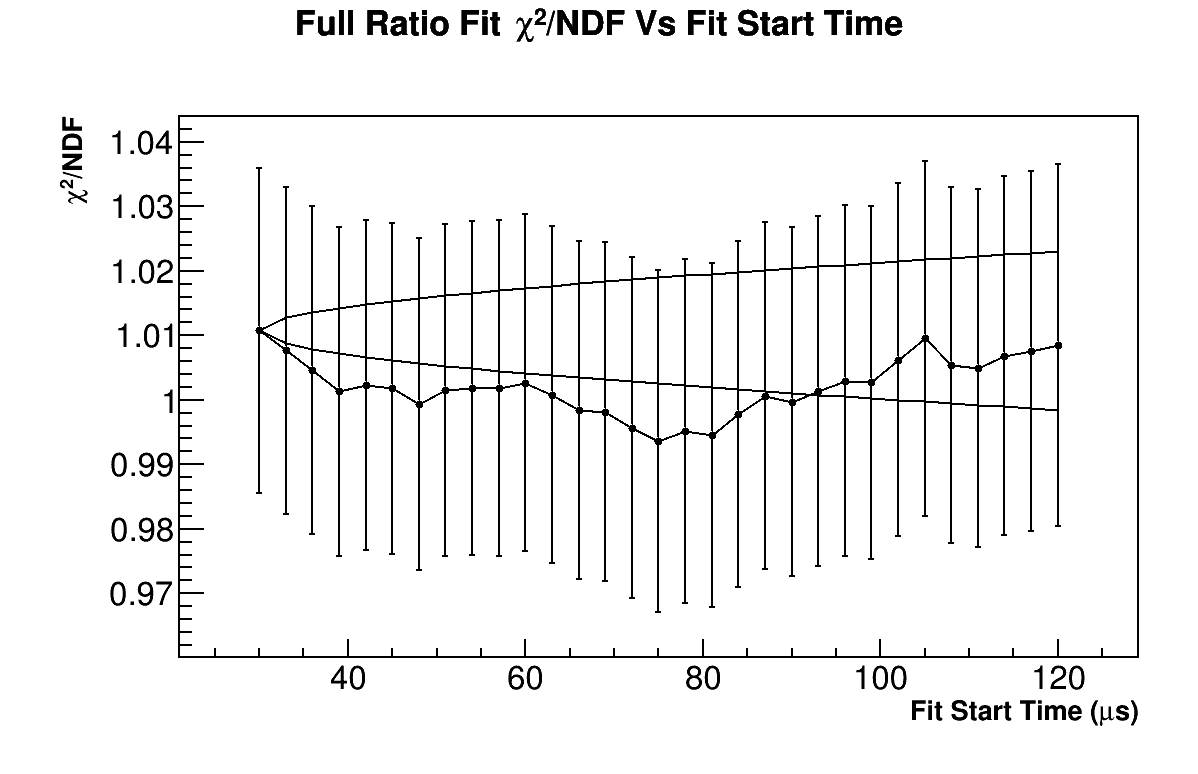
\includegraphics[width=\textwidth]{RatioCBO_Chi2NDF_Vs_FS_canv-Seed12}
	    \caption{Seed 3}
    \end{subfigure}
    \begin{subfigure}[t]{0.45\textwidth}
	    \centering
		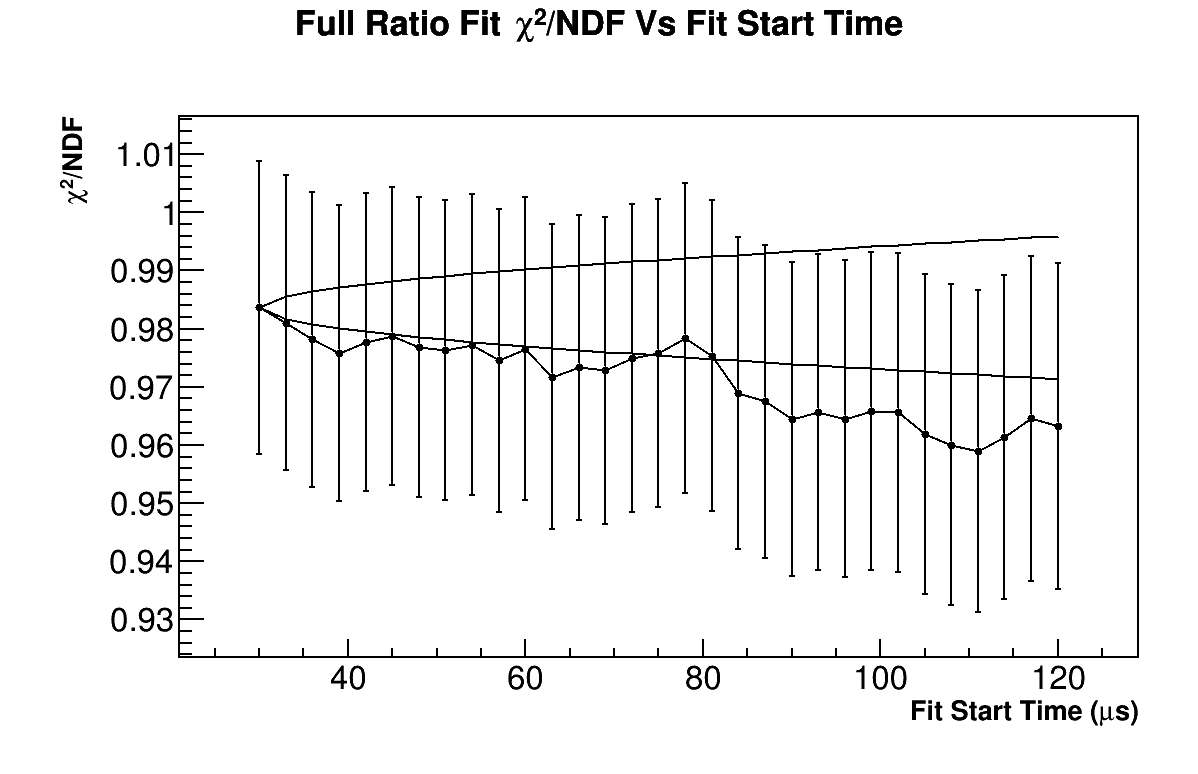
\includegraphics[width=\textwidth]{RatioCBO_Chi2NDF_Vs_FS_canv-Seed18}
	    \caption{Seed 4}
    \end{subfigure}% %you need this % here to add spacing between subfigures
\caption[RandomSeedFitStartScans]{Fit start time scans for the \chisq for four random seeds of the randomization of the same dataset. Compare to Figure \ref{fig:RatioCBO_Chi2NDF_Vs_FS_canv}. Note how the scans rise and fall at different points but are all consistent with the statistical bands.}
\label{fig:RandomSeedFitStartScans}
\end{figure}



\section{Final Systematic Uncertainty Table}

\section{Final Results}
